\section{Функционал шаардлагууд}
\begin{table}[h]
	\centering
	\begin{tabular}{ |p{2cm}|p{13cm}| }
		ФШ 100 & Систем нь хэрэглэгчдэд лиценз баталгаажуулахын тулд янз бүрийн форматтай цахим баримт бичгүүдийг (жишээлбэл, .doc, .pdf, .xls гэх мэт) байршуулахыг зөвшөөрөх ёстой. \\ \hline
      ФШ 200 & Систем нь аюулгүй хэйшлэх алгоритм ашиглан байршуулсан файл бүрт  эсвэл хэйш үүсгэх ёстой. \\ \hline
		ФШ 300 & Систем нь хэрэглэгчдийг баримт бичигт гарын үсэг зурах, баталгаажуулахаас өмнө баталгаажуулах ёстой. Үүнийг хэрэглэгчийн нэр/нууц үг, олон хүчин зүйлийн баталгаажуулалт эсвэл бусад аюулгүй аргуудаар хийж болно. \\ \hline
		ФШ 400 & Систем нь блокчэйнээр дамжуулан тодорхой файлтай холбоотой лицензийн үнэн зөв, хүчинтэй эсэхийг шалгах боломжтой байх ёстой. \\ \hline
		ФШ 500 & Систем нь файлтай холбоотой мэдээллийг хадгалах, сэргээх зорилгоор блокчейн сүлжээтэй (жишээ нь, Ethereum нэгдсэн байх ёстой. \\  \hline
		ФШ 600 & Лицензийн баталгаажуулалт, эзэмшил, файлын мета өгөгдлийг удирдахын тулд ухаалаг гэрээг боловсруулж, блокчэйнд байршуулна. \\  \hline
		ФШ 700 & Систем нь лицензийн баталгаажуулалтын гүйлгээний ил тод байдал, хяналтыг сайжруулахын тулд блокчейн event болон log бүртгэлийг ашиглах ёстой. \\  \hline
	\end{tabular}
   \caption{Функциональ шаардлага}
\end{table}


\section{Функционал бус шаардлагууд}
\begin{table}[h!]
	\centering
	\begin{tabular}{ |p{2cm}|p{13cm}| }
		\hline
		ФБШ 100 & Систем нь GDPR эсвэл HIPAA гэх мэт холбогдох бүх мэдээллийн аюулгүй байдал, нууцлалын дүрэм журмыг дагаж мөрдөх ёстой. Гарын үсэг, баримт бичиг зэрэг бүх өгөгдөл шифрлэгдсэн байх ёстой. \\ \hline
		ФБШ 200 & Систем нь гүйцэтгэлийн бууралтгүйгээр олон тооны хэрэглэгчид болон баримт бичгүүдийг зохицуулах чадвартай байх ёстой. \\ \hline
		ФБШ 300 & Үүлэн үйлчилгээ нь хамгийн бага зогсолттой, 24/7 цагийн турш ашиглах боломжтой байх ёстой. Үйлчилгээний түвшний гэрээ (SLA) нь дор хаяж 99.9\% ажиллах хугацааг баталгаажуулах ёстой.     \\ \hline
		ФБШ 400 & Систем нь хүлээн зөвшөөрөгдсөн тодорхой хугацааны дотор гарын үсэг үүсгэх, баталгаажуулах хүсэлтийг хурдан боловсруулах чадвартай байх ёстой.                                             \\ \hline
		ФБШ 500 & Систем нь янз бүрийн техникийн чадвартай хэрэглэгчдэд үүнийг үр дүнтэй ашиглах боломжийг олгодог хэрэглэгчдэд ээлтэй интерфэйстэй байх ёстой.                                             \\ \hline
		ФБШ 600 & Үүлэн үйлчилгээ нь янз бүрийн үйлдлийн систем, хөтөч, төхөөрөмжтэй нийцтэй байх ёстой.                                                                                                    \\  \hline
		ФБШ 700 & Энэ систем нь гамшгийн үед өгөгдөл алдагдахгүй байхын тулд найдвартай нөөцлөх, сэргээх механизмтай байх ёстой.                                                                            \\ \hline
		ФБШ 800 & Систем нь Европ дахь eIDAS эсвэл АНУ-ын ESIGN хууль зэрэг тоон гарын үсгийн хууль тогтоомж, дүрэм журамд нийцсэн байх ёстой.                                                              \\ \hline
	\end{tabular}
   \caption{Функциональ бус шаардлага}
\end{table}

% \section{Use-case диаграм}
% \begin{figure}[h]
% 	\centering
% 	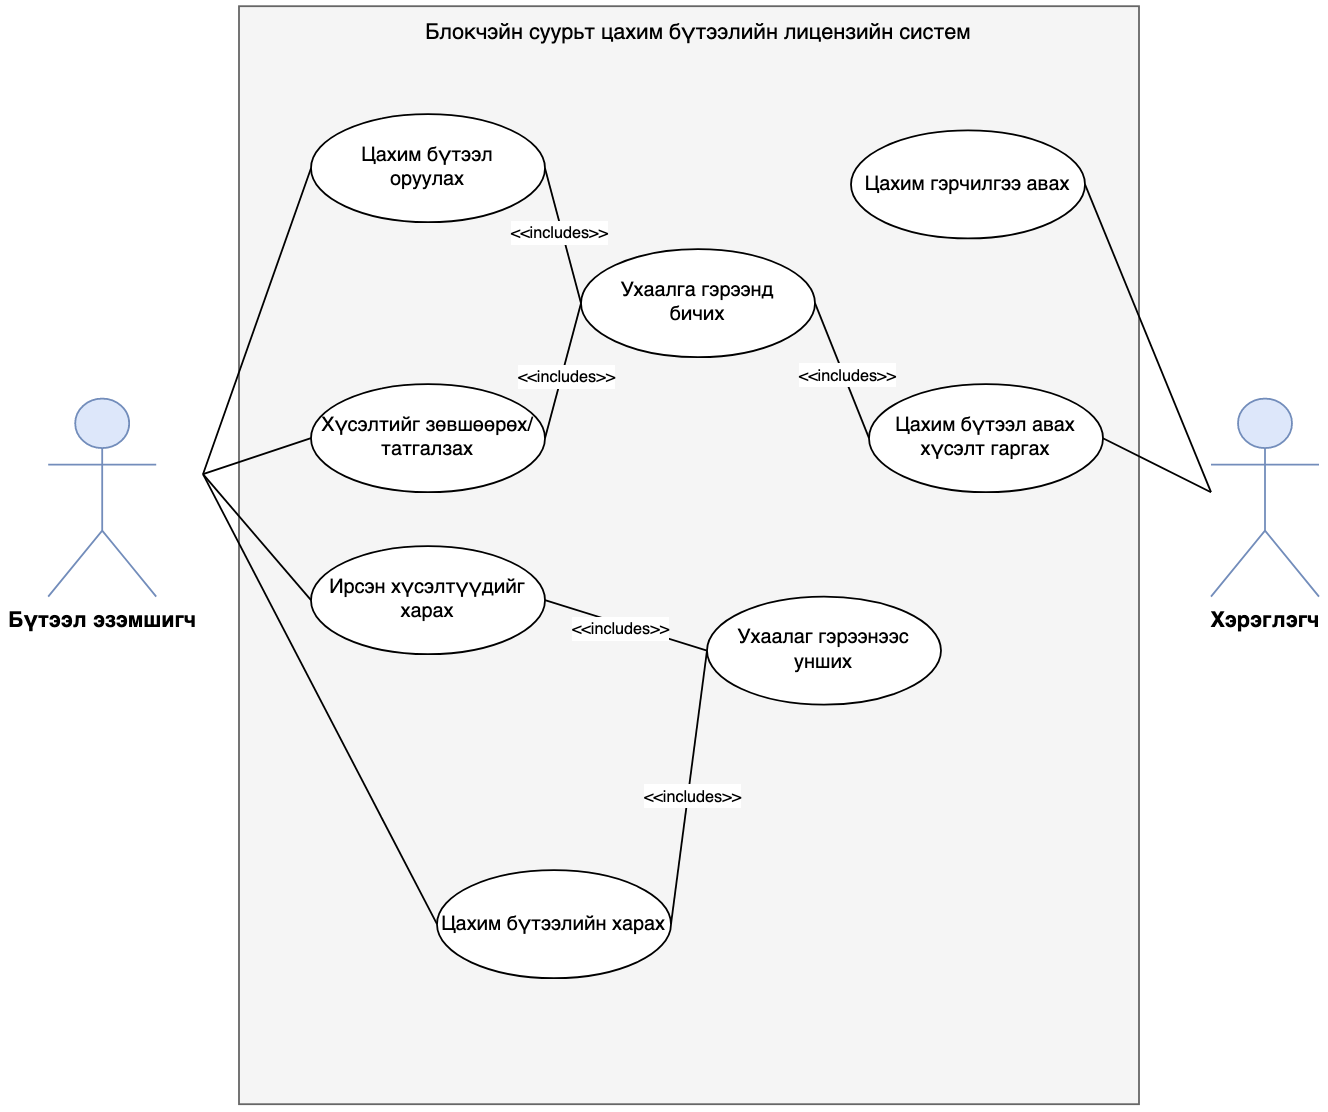
\includegraphics[scale=0.3]{src/images/usecase.png}
% 	\caption{Use-case диаграм}
% \end{figure}
